\documentclass[documentclass]{jsarticle}
\usepackage[top=25truemm,bottom=25truemm,left=20truemm,right=20truemm]{geometry}
\usepackage{listings, jlisting, color}
\usepackage[dvipdfmx]{graphicx}
\usepackage{pdfpages}
\usepackage{amsmath}
\usepackage{amssymb, latexsym}
\usepackage{mathtools}
\usepackage{multirow}
\usepackage{color}
\usepackage{ulem}
\usepackage{here}
\usepackage{wrapfig}
\usepackage{tikz}
\usepackage{tcolorbox}
\tcbuselibrary{breakable, skins, theorems}

% 使用する関数の宣言
% (最低限これさえ宣言していれば十分だと思われるものを書いています)
\usetikzlibrary{intersections, calc, arrows, positioning, arrows.meta}


\newcommand{\Add}[1]{\textcolor{red}{#1}}
\newcommand{\Erase}[1]{\textcolor{red}{\sout{\textcolor{black}{#1}}}}
\newcommand{\ctext}[1]{\raise0.2ex\hbox{\textcircled{\scriptsize{#1}}}}

\lstset{
  basicstyle={\small},
  breaklines=true,
  frame=single,
  tabsize=3,
  numbers=left
}

\begin{document}
\title{ソフトウェア設計演習 最終レポート}
\author{222C1021 今村優希}
\maketitle

%\tableofcontents
\clearpage

\newpage

\section{今回のシステム}

今回は下記仕様の「Live Campus」のようなシステムをモデル化する.
システムの大まかな概要を下記に記す.

\begin{tcolorbox}
  \begin{itemize}
    \item 学生は毎学期ごとに、システムから履修登録を行い、許可された講義を受講する。
    履修の可否は、学修細則に基づきシステムが判断する。
    各学期ごとに履修できる科目数には上限があり、同じ時限に重複した科目を履修することはできない。
    \item 学生は、履修登録期間内には何度でも登録、削除、修正(更新)を行うことが出来る。
    \item 学生は、登録した科目と登録可能な科目の時間割をそれぞれ見ることが出来る。
    \item 学生は、自身のこれまでの成績を確認することができる。
    \item 科目には、必修と選択があり、不合格の必修科目があれば履修登録時にシステムが提示し、履修を促す。
    \item 教員は、複数の科目を担当することがあり、システムから各科目の成績を報告する。
    なお、科目担当者は1名とする。
    \item システムは、成績報告期限までに報告していない教員に督促メールを送る。
    なお、成績報告期限の1週間前に成績報告していない教員には、期限を知らせるメールを送るものとする。
  \end{itemize}
\end{tcolorbox}

\section{設計の作成手順}
今回の設計では,分析モデルを作成した後に,設計モデルを作成する手順を取った.

分析モデルでは以下のUML図を作成した.
各UML図が作成し終わると,レビューを行い,後の工程に大きな影響が出ないように工夫を行った.
\begin{itemize}
  \item ユースケース図
  \item ユースケース記述
  \item クラス図
  \item シーケンス図
  \item アクティビティ図
  \item ステートマシン図
\end{itemize}

これらの図を作成し,分析が一定できると,設計モデルの作成に着手した.
設計モデルでは,パターンの適用を駆使し,システムがより現実的になるよう改変を加えた.


\newpage

\section{ユースケース図}
\subsection*{概要}
システムの概要を把握するためにユースケース図を作成した.
今回のシステムの内容から,必要なアクターは
\begin{itemize}
  \item 学生
  \item 教員
\end{itemize}
であると考えた.

学生は「システムにログイン」,「履修登録,削除」等の直接行うユースケースを作成した.
「履修を促す」というシステム側から行われるユースケースを関連付けている.

教員は「システムにログイン」,「成績の報告をする」というユースケースを作成した.
また,学生と同様に成績報告に関する通知を行うユースケースを関連付けている.

\subsection*{レビュー結果}
ユースケース「履修の可否を確認する」に関して,「学生」と関連をつけた方が良いということで,「履修登録する」にincludeで関連付けた.
また,ユースケース「ログインする」が必要だと思ったので,作成し,他のユースケースと関連をつけた.

概要から「履修修正」という要件があったが,今回のシステムでは履修削除と履修登録を組み合わせて行うと考えた.

\subsection*{作成した図}
レビュー等を通して作成したユースケースが図\ref*{fig:3-1}である.
%ユースケース図の作成結果
\begin{figure}[H]
  \begin{center}
    \includegraphics*[scale=0.5]{figure/3-1.png}
  \end{center}
  \caption{ユースケース図}
  \label{fig:3-1}
\end{figure}

\newpage

\section{ユースケース記述}
\subsection*{概要}
上記で作成したユースケースすべてに対してユースケース記述の作成を行った.
ユースケースそれぞれに対して基本系列を作成し,加えて代替系列が必要なユースケースでは適宜作成を行った.

\subsection*{作成した図}
\subsubsection*{1.学生用にログインする}
\begin{figure}[H]
  \includegraphics*[scale=0.4]{figure/4-1.png}
\end{figure}

\subsubsection*{2.履修登録する}
\begin{figure}[H]
  \includegraphics*[scale=0.4]{figure/4-2.png}
\end{figure}

\subsubsection*{3.履修削除する}
\begin{figure}[H]
  \includegraphics*[scale=0.4]{figure/4-3.png}
\end{figure}

\subsubsection*{4.履修修正する}
\begin{figure}[H]
  \includegraphics*[scale=0.4]{figure/4-4.png}
\end{figure}

\subsubsection*{5.時間割を確認する}
\begin{figure}[H]
  \includegraphics*[scale=0.4]{figure/4-5.png}
\end{figure}

\subsubsection*{6.成績を確認する}
\begin{figure}[H]
  \includegraphics*[scale=0.4]{figure/4-6.png}
\end{figure}

\subsubsection*{7.未習得の履修を促す}
\begin{figure}[H]
  \includegraphics*[scale=0.4]{figure/4-7.png}
\end{figure}

\subsubsection*{8.教員用にログインする}
\begin{figure}[H]
  \includegraphics*[scale=0.4]{figure/4-8.png}
\end{figure}

\subsubsection*{9.成績の報告をする}
\begin{figure}[H]
  \includegraphics*[scale=0.4]{figure/4-9.png}
\end{figure}

\subsubsection*{10.成績報告督促を送る}
\begin{figure}[H]
  \includegraphics*[scale=0.4]{figure/4-10.png}
\end{figure}

\subsubsection*{11.成績報告期限メールを送る}
\begin{figure}[H]
  \includegraphics*[scale=0.4]{figure/4-11.png}
\end{figure}

\subsubsection*{12.履修の可否を確認する}
\begin{figure}[H]
  \includegraphics*[scale=0.4]{figure/4-12.png}
\end{figure}

\newpage

\section{クラス図}
\subsection*{概要}
全体のクラス図は図\ref*{fig:5-1}である.
この図に対して,学生,教員それぞれに関係するクラスで分割して物で詳細な関係を分析した.
そのため,\ref*{fig:5-1}における関係に重複度が内藤の不具合があるが,それは分割した詳細な図で行っているため問題ないと考えている.
\begin{figure}[H]
  \begin{center}
    \includegraphics*[scale=0.3]{figure/5-1.png}
  \end{center}
  \caption{ユースケース図}
  \label{fig:5-1}
\end{figure}

以下でそれぞれのクラスに関して何を行うためのものであるかを示す.

\paragraph*{学生クラス}
学生の名前や学生番号が属性として保存されている.
科目の選択や時間割を確認等の動作を行う.

\subsection*{作成したもの}

%クラス図の表示(未完成なので用修正)
\begin{figure}[H]
  \begin{center}
    \includegraphics*[scale=0.4]{figure/5-2.png}
  \end{center}
  \caption{ユーザーに関するクラス図}
  \label{fig:5-2}
\end{figure}

\begin{figure}[H]
  \begin{center}
    \includegraphics*[scale=0.4]{figure/5-3.png}
  \end{center}
  \caption{学生に関するクラス図}
  \label{fig:5-3}
\end{figure}

\begin{figure}[H]
  \begin{center}
    \includegraphics*[scale=0.4]{figure/5-4.png}
  \end{center}
  \caption{教員に関するクラス図}
  \label{fig:5-4}
\end{figure}


\newpage

\section{シーケンス図}
\subsection*{概要}
作成したシーケンス図は,
\begin{itemize}
  \item 
\end{itemize}


\subsection*{作成した図}

%シーケンス図の表示
\begin{figure}[H]
  \centering
  \begin{minipage}[b]{0.49\columnwidth}
      \centering
      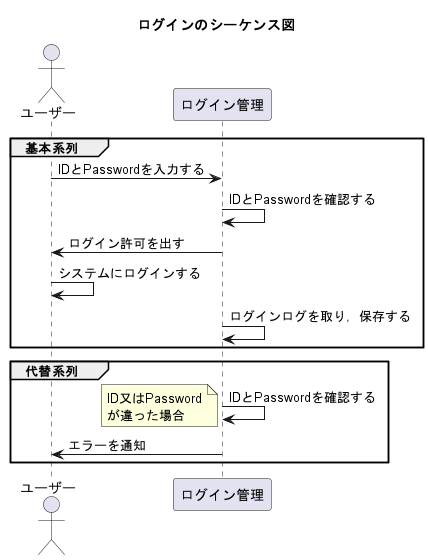
\includegraphics[width=1.0\columnwidth]{figure/6-1.png}
      \caption{ログイン時のシーケンス図}
      \label{fig:6-1}
  \end{minipage}
  \begin{minipage}[b]{0.49\columnwidth}
      \centering
      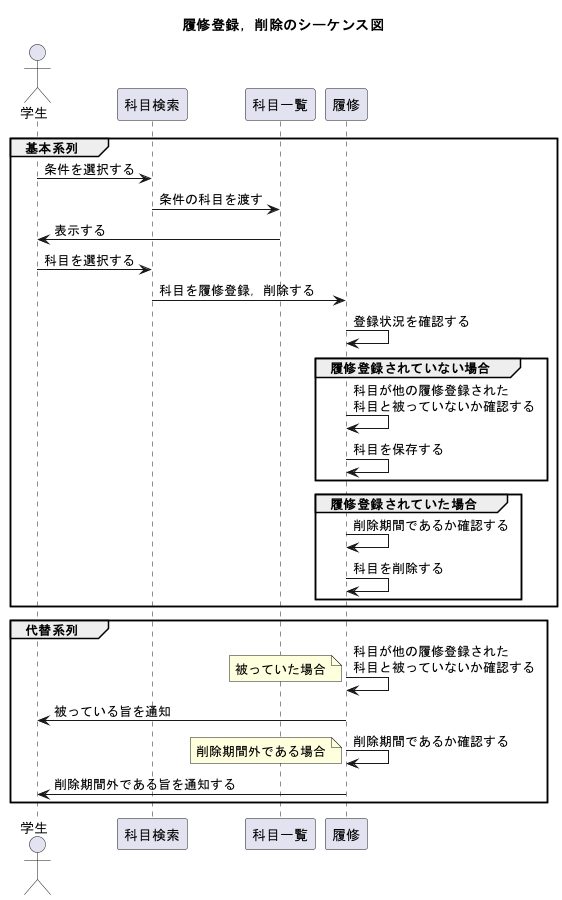
\includegraphics[width=1.0\columnwidth]{figure/6-2.png}
      \caption{履修登録,履修削除のシーケンス図}
      \label{fig:6-2}
  \end{minipage}
\end{figure}

\begin{figure}[H]
  \centering
  \begin{minipage}[b]{0.49\columnwidth}
      \centering
      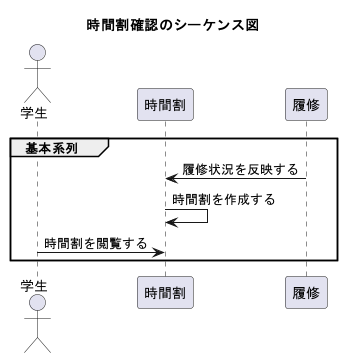
\includegraphics[width=1.0\columnwidth]{figure/6-3.png}
      \caption{時間割確認のシーケンス図}
      \label{fig:6-3}
  \end{minipage}
  \begin{minipage}[b]{0.49\columnwidth}
      \centering
      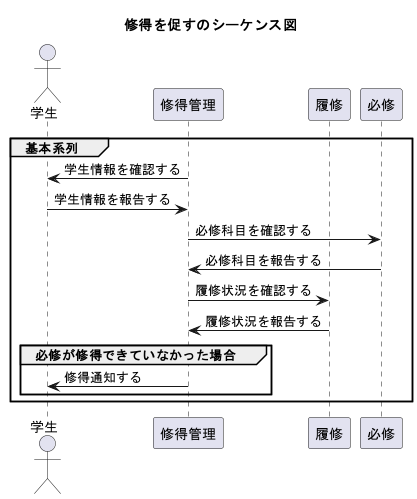
\includegraphics[width=1.0\columnwidth]{figure/6-5.png}
      \caption{修得を促すシーケンス図}
      \label{fig:6-5}
  \end{minipage}
\end{figure}

\begin{figure}[H]
  \begin{center}
    \includegraphics*[scale=0.5]{figure/6-4.png}
  \end{center}
  \caption{ユースケース図}
  \label{fig:6-4}
\end{figure}

\begin{figure}[H]
  \begin{center}
    \includegraphics*[scale=0.5]{figure/6-6.png}
  \end{center}
  \caption{ユースケース図}
  \label{fig:6-6}
\end{figure}


\newpage

\section{アクティビティ図}
\subsection*{概要}
作成したアクティビティ図は「バスの位置を確認する」と「バスの位置を記録する」である.


\subsection*{作成した図}
\begin{figure}[H]
  \begin{center}
    \includegraphics*[scale=0.4]{figure/7-1.png}
  \end{center}
  \caption{ユースケース図}
  \label{fig:7-1}
\end{figure}

\begin{figure}[H]
  \begin{center}
    \includegraphics*[scale=0.4]{figure/7-2.png}
  \end{center}
  \caption{ユースケース図}
  \label{fig:7-2}
\end{figure}

\begin{figure}[H]
  \centering
  \begin{minipage}[b]{0.49\columnwidth}
      \centering
      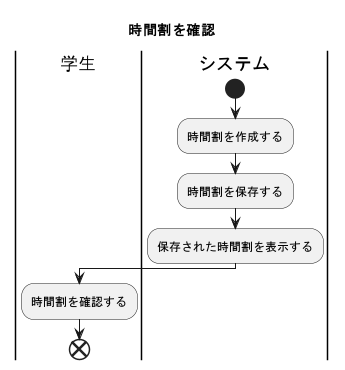
\includegraphics[width=0.9\columnwidth]{figure/7-3.png}
      \caption{ログイン時のシーケンス図}
      \label{fig:7-3}
  \end{minipage}
  \begin{minipage}[b]{0.49\columnwidth}
      \centering
      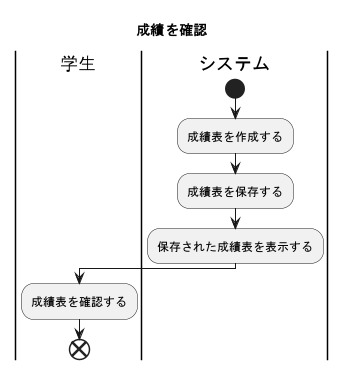
\includegraphics[width=0.9\columnwidth]{figure/7-4.png}
      \caption{履修登録,履修削除のシーケンス図}
      \label{fig:7-4}
  \end{minipage}
\end{figure}

\begin{figure}[H]
  \centering
  \begin{minipage}[b]{0.49\columnwidth}
      \centering
      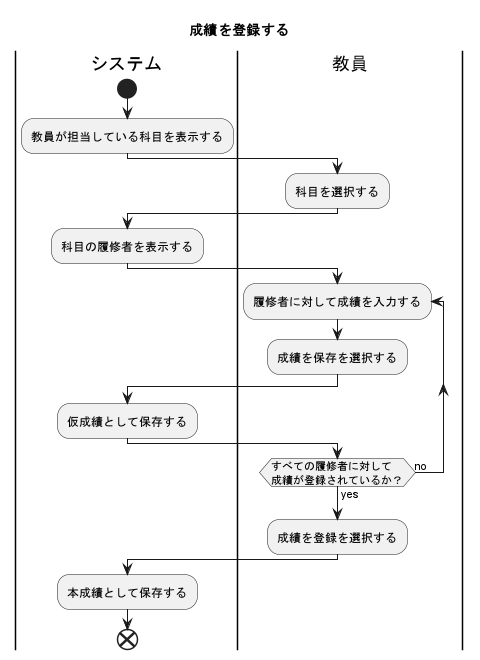
\includegraphics[width=1.0\columnwidth]{figure/7-5.png}
      \caption{ログイン時のシーケンス図}
      \label{fig:7-5}
  \end{minipage}
  \begin{minipage}[b]{0.49\columnwidth}
      \centering
      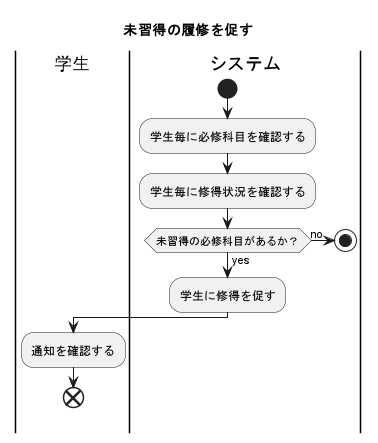
\includegraphics[width=1.0\columnwidth]{figure/7-6.png}
      \caption{履修登録,履修削除のシーケンス図}
      \label{fig:7-6}
  \end{minipage}
\end{figure}

\begin{figure}[H]
  \begin{center}
    \includegraphics*[scale=0.4]{figure/7-7.png}
  \end{center}
  \caption{ユースケース図}
  \label{fig:7-7}
\end{figure}
\newpage

\section{ステートマシン図}
\subsection*{概要}
今回のシステムにおいて,「成績」の報告に関してステートが変化することからステートマシン図を作成した.
成績は,「未登録状態」→「仮成績」→「本成績」の順で変化する.
その図を図\ref*{fig:8-1}で示す.

\subsection*{作成した図}
\begin{figure}[H]
  \begin{center}
    \includegraphics*[scale=0.6]{figure/8-1.png}
  \end{center}
  \caption{}
  \label{fig:8-1}
\end{figure}

\newpage

\section{設計モデルのクラス図}
作成したクラス図に対して,パターンを導入する等の設計モデルの作成を行った.

\section{まとめ}


\end{document}